% Modelo de Dissertação em Latex para o PPG em Engenharia Elétrica - Sistemas Eletrônicos da UERJ
% Este modelo foi adaptado da versão disponibilizada no site da Engenharia Elétrica da UERJ
% http://www.pel.uerj.br/publico/Modelo_LaTeX_Dissertacao_UERJ.rar
% http://www.pel.uerj.br/defesas/
% 
%
% 
%
% 
% Atualizações:
% Felipe M. - 20/06/2012
% Fernando Lima - 15/07/2015
%





\documentclass[a4paper,12pt,oneside,openany]{uerj}

\usepackage[english,brazil]{babel}
%\usepackage[latin1]{inputenc}
\usepackage[utf8]{inputenc}
\usepackage{enumerate}
\usepackage{cite}
\usepackage{epsf,epsfig,./packages/psfig}
\usepackage{./packages/pagina}
\usepackage{indentfirst}
\usepackage{theorem}
\usepackage{fancyhdr}
\usepackage{setspace}
\usepackage{boxedminipage}
\usepackage{float}
\usepackage{makeidx}
\usepackage{amsmath}
\usepackage[hidelinks]{hyperref}
\usepackage{listings}
\usepackage{xcolor}




%%%%%% Definições %%%%%%%
\newtheorem{deff}{Definição}[section]
\numberwithin{equation}{chapter}

\theoremstyle{plain}

\bibliographystyle{./bib/abnt-num}



%%%%% DOC %%%%%%%%%%%%


\makeindex


\begin{document}


%%% Modifique aqui seu Nome, título do trabalho e data

\newcommand{\setNomeAluno}{Fernando de Oliveira Lima}
\newcommand{\setTitulo}{Sistema Escalável para Aplicações de Internet das Coisas utilizando MQTT}
\newcommand{\setLocationDate}{Rio de Janeiro\\2018} % Coloque aqui a localização e data
\newcommand{\setApprovalDate}{28 de Agosto 2018}


\hypersetup{
    colorlinks,
    citecolor=black,
    filecolor=black,
    linkcolor=black,
    urlcolor=black,
    linktoc=all,
}

\thispagestyle{empty}\begin{titlepage}
\begin{center}

	\vspace{-0.5cm}

  \begin{figure}[hbt!]
		\begin{flushleft}
		   
\includegraphics[width=3.44cm,height=3.17cm]{./01_Pre_textuais/figures/logo_uerj_pb.png}
		\end{flushleft}
	\end{figure}
	\vspace{-4cm}

  \hspace{2cm}\large{\textbf{Universidade do Estado do Rio de Janeiro}}\\
  \hspace{2cm}\large{Centro de Tecnologia e Ciências}\\
  \hspace{2cm}\large{Faculdade de Engenharia}\\

  \hspace{2cm}\large{}\\
  \hspace{2cm}\large{}\\
  \hspace{2cm}\large{}\\
  \hspace{2cm}\large{}\\

  \par
  \large{\setNomeAluno}

  \hspace{2cm}\large{}\\
  \hspace{2cm}\large{}\\
  \hspace{2cm}\large{}\\
  \hspace{2cm}\large{}\\


  \par
  \large\textbf{\setTitulo}


  \par\vfill
  \setLocationDate

\end{center}
\end{titlepage}
\pagebreak\thispagestyle{empty}\begin{center}

\setNomeAluno
% \vfill
\vspace{2cm}

\textbf{\setTitulo}

\vspace{1.0cm}

\begin{figure}[hbt!]
\begin{center}

\includegraphics[width=10.48cm,height=10.8cm]{./01_Pre_textuais/figures/logo_uerj_gnd_pb.png}
\end{center}
\end{figure}

\vspace{-9cm}
\begin{flushright}
\parbox{8cm}{
\singlespacing{Projeto de Graduação apresentado, como requisito parcial para obtenção do grau de Engenheiro Eletricista, á Faculdade de Engenharia, da Universidade do Estado do Rio de Janeiro. Ênfase: Sistemas Eletrônicos.}
}
\end{flushright}

\vspace{4.0cm}


\begin{table}[h!]
\centering
\begin{tabular}{ll}
Orientadores: & Prof. Michel Tcheou, DSc\\
					& Prof. Lisandro Lovisolo, DSc\\
\end{tabular}
\end{table}


\par\vfill
%\vspace{2cm}

\setLocationDate
\end{center}
\pagebreak\thispagestyle{empty}% Depois de preparar seu trabalho, você deverá enviá-lo para a Biblioteca CTC/B para avaliação do formato e elaboração da Ficha catalográfica.
% Com a ficha pronta (fornecida pela Biblioteca), você poderá alterar este trecho do trabalho em definitivo.
%
% Para este processo, enviei a dissertação em PDF para o email: ctcb.uerj.bdtd@gmail.com (Tratei de todos os detlahes com a Sra. Márcia)
% Qualquer dúvida, veja os contatos da Biblioteca no site da Rede Sirius: http://www.rsirius.uerj.br/
% 


\begin{titlepage}
	\begin{center}
\vfill
\singlespacing
	\vspace*{95mm}
	{CATALOGAÇÃO NA FONTE\\ \vspace{1.5mm}
	UERJ\,/\,REDE SIRIUS\,/\,BIBLIOTECA CTC/B}\\
	\vspace{1.5mm}
	\begin{boxedminipage}{140mm}
	\begin{minipage}{5mm}
		\vspace{-84mm}
		S237
	\end{minipage}
	\hfill
	\raisebox{8.5mm}{
	\begin{minipage}[top]{115mm}
		\vspace*{5mm}

		de Oliveira Lima, Fernando\\
		\phantom{XX}\setTitulo\,/\,\setNomeAluno -- 2018.\\
		\phantom{XX}\pageref{LastPage}\,f.\\
		\phantom{XX}\\
		\phantom{XX}Orientadores: Michel Pompeu Tcheou, Lisandro Lovisolo.\\
       		\phantom{XX}Projeto de Graduação -- Universidade do Estado do Rio de Janeiro, Faculdade de Engenharia.\\
		\phantom{XX} Bibliografia: p.43\\
		\phantom{XX} \\
		\phantom{XX} Texto a ser informado pela biblioteca
	\end{minipage}}
	\vspace*{5mm}
	\begin{flushright}
	 CDU~621:528.8
	\end{flushright}
    \vspace{1mm}
	\end{boxedminipage}\\
	\end{center}
%
	Autorizo, apenas para fins acadêmicos e científicos, a reprodução total ou parcial desta dissertação, desde que citada a fonte.\\
	\noindent
	\begin{tabular}{ccc}
	\phantom{XXXXXXXXXXXXXXXXXXXXXXXXXXXXXX}&	 \phantom{XX}	&	\phantom{XXXXXXXXXXXXXXXX}	\\
	\phantom{XXXXXXXXXXXXXXXXXXXXXXXXXXXXXX}&	 \phantom{XX}	&	\phantom{XXXXXXXXXXXXXXXX}	\\
	\cline{1-1}\cline{3-3}
	Assinatura &		&	Data
	\end{tabular}
\end{titlepage} 
\pagebreak\thispagestyle{empty}\addtocounter{page}{+1}
\begin{center}

\setNomeAluno

\vspace{1cm}

\textbf{\setTitulo}

\end{center}

\vspace{.4cm}

\begin{flushright}
\parbox{8cm}{
\singlespacing{Trabalho de Conclusão de Curso apresentado, como requisito parcial para obtenção do título de Bacharel em Engenharia Elétrica ênfase em Sistemas Eletrônico, da Universidade do Estado do Rio de Janeiro.}
}
\end{flushright}

\vspace{.6cm}


% insira abaixo a data de sua defesa
% Caso não tenha defendido ainda, deixe em branco

\noindent Aprovado em: \setApprovalDate

\noindent Banca Examinadora:


%
%
% Os professores da UERJ DEVEM ser citados primeiro, independente de quem seja o orientador.
%
%



\vspace{.7cm}

\begin{flushright}
\parbox{12cm}{

\singlespacing

\hrulefill \\

\vspace{-.4cm}
Prof. Dr. Michel Pompeu Tcheou (Orientador)
\newline
Departamento de Eletrônica e Telecomunicações  da UERJ
\vspace{.7cm}

\hrulefill \\

\vspace{-.4cm}
Prof. Dr. Lisandro Lovisolo (Orientador)
\newline
Departamento de Eletrônica e Telecomunicações  da UERJ
\vspace{.7cm}


\hrulefill \\

\vspace{-.4cm}
Prof. Dr. Nome do Professor 3
\newline
Universidade Federal do Rio de Janeiro - UFRJ - COPPE
\vspace{.7cm}

\hrulefill \\

\vspace{-.4cm}
Prof. Dr. Nome do Professor 4
\newline
Instituto de Geociências da UFF
\vspace{.7cm}
}
\end{flushright}
\vfill

\begin{center}
\setLocationDate
\end{center}

\pagebreak\thispagestyle{empty}\begin{center}
\textbf{DEDICATÓRIA}
\end{center}

$\!$\\

%\vspace{1cm}

Aqui entra sua dedicatória.




\pagebreak\thispagestyle{empty}\begin{center}
\textbf{AGRADECIMENTO}
\end{center}

$\!$\\

Agradeço aos amigos e aos não tão amigos, que igualmente fizeram parte da minha evolução como ser humano e cidadão. Todas as pessoas que passaram na minha vida contribuíram um pouco para esse momento, não há como saber onde todas estão, mas se um dia lerem esse texto, quero que saiba que eu agradeço a companhia e o aprendizado.

Não poderia ficar de fora, é claro, todos aqueles que de Alguma forma foram meus mentores. Meus professores ao longo da vida, em especial os dois orientadores desse projeto, já os conheço a quase sete anos, fizeram parte da minha formação, me deram oportunidades e ajudaram a concretizar esse trabalho. Agradeço de coração, que mais oportunidades de nos encontrar surjam, e desejo todo o sucesso possível e uma vida feliz e confortável.

Fica meu agradecimento aqui também para essa instituição linda e maravilhosa, que não é fácil de lidar, muitas vezes pareceu que ia nos abandonar, mas trouxemos ela de volta, cada um com sua parte. Obrigado UERJ, por uma parte inesquecível da minha vida e por todas as pessoas que conheci dentro deste universidade.

E se você estiver lendo esse texto, sim, você mesmo leitor! Agradeço seu prestígio, mesmo se você tiver ignorado completamente esta parte. Espero que tenha aprendido um pouco. O texto é para Ciência, para a Tecnologia e para você.

 
%\pagebreak\thispagestyle{empty}\input{./01_Pre_textuais/Epigrafe}    % não coloquei epígrafe no meu trabalho, mas fica aqui a chamada comentada.
\pagebreak\thispagestyle{empty}\begin{center}
\textbf{RESUMO}
\end{center}

%
% O resumo deve ser organizado em apenas um parágrafo mesmo.
% O número de folha é o número de páginas do PDF -2. Isto ocorre pois na versão final (capa dura) a capa é removida e as duas primeiras páginas são impressas em uma % folha apenas (frente e verso).
%

$\!$\\

\hspace{-1.3cm}\textbf{LIMA}, Fernando \textit{\setTitulo}. 105 f. Trabalho de Conclusão de Curso~(Engenharia Elétrica ênfase em Sistemas Eletrônicos) - Faculdade de Engenharia, Universidade do Estado do Rio de Janeiro (UERJ), Rio de Janeiro, 2018.

\vspace{.2cm}

No meio da revolução dos dados, cresce o interesse em sistemas de comunicação entre máquinas e sistemas de compartilhamento e visualização de dados  sobre dispositivos, seja numa fábrica ou em residências. Este trabalho apresenta um sistema para aplicações de internet das coisas(IoT) utilizando MQTT, um protocolo de aplicação para comunicação entre dispositivos que enviam dados telemétricos. É  a \textit{língua franca} para publicação de dados telemétricos via TCP/IP, com persistência de dados em banco MongoDB. O sistema englobará todos os setores de aquisição dos dados a camada de aplicação em consoles, com o objetivo de facilitar a implementação de aplicações eficientes em cada cenário.

\vspace{1cm}

\hspace{-1.3cm}Keywords: IoT, MQTT, industry .
\pagebreak\thispagestyle{empty}\begin{center}
\textbf{ABSTRACT}
\end{center}

$\!$\\

% O resumo em inglês deve ser organizado em apenas um parágrafo mesmo.

In the verge of the data revolution, a growing interest in communication sytems between machines and the sharing systems of telemetric data on devices rises, whether in a factory or in a residence. This work presents a system for Internet applications of things (IoT) using MQTT, an application protocol for communication between devices that shares telemetri data . It is the \textit{língua franca} for publishing telemetric data via TCP / IP, with data persistion using MongoDB. The system will  encompass all sectors of data acquisition to the application layer in consoles, facilitating implementations of applications in each scenario.

\vspace{1cm}

\hspace{-1.3cm}Keywords: IoT, MQTT, industry .

\fancypagestyle{plain}{
\fancyhf{} % clear all header and footer fields
\renewcommand{\headrulewidth}{0pt}
\renewcommand{\footrulewidth}{0pt}}
\pagestyle{plain}

\pagebreak

\def\listfigurename{LISTA DE FIGURAS}\listoffigures
\def\listtablename{LISTA DE TABELAS}\listoftables

% Caso tenha códigos
\renewcommand{\lstlistingname}{Códigos}
\renewcommand{\lstlistlistingname}{Lista de \lstlistingname}\lstlistoflistings

\newpage

\begin{center}
\textbf{LISTA DE SIGLAS}
\end{center}
$\!$\\

\begin{tabular}{lll}
IoT & \hspace{1cm} & Internet das Coisas \\
NB &\hspace{1cm} &  Narrow Band Networks \\
A/D & \hspace{1cm} & Analógico-Digital \\
DB &  \hspace{1cm} & Banco de Dados \\
IaaS & \hspace{1cm} & Infrastructure as a Service \\
MCU & \hspace{1cm} & Micro-Controller Unit \\
\end{tabular}
    % não coloquei LISTA DE SIGLAS no meu trabalho, mas fica aqui a chamada comentada.
\def\contentsname{SUMÁRIO}\tableofcontents

\fancypagestyle{plain}{
\fancyhf{} % clear all header and footer fields
\fancyhead[R]{\thepage}
\setlength{\voffset}{-1cm}
\setlength{\headsep}{1cm}
\renewcommand{\headrulewidth}{0pt}
\renewcommand{\footrulewidth}{0pt}}

\pagestyle{plain}

\pagebreak
\addcontentsline{toc}{chapter}{\hspace{1.7cm}\bfseries INTRODUÇÃO}
\noindent\textbf{INTRODUÇÃO}
$\!$\\

O cenário atual do desenvolvimento tecnológico encontra-se no meio de uma quarta revolução industrial. Nunca se produziu tantos dados e utilizou-se redes como a própria internet para propaga-los. É de se esperar que tanto o cenário acadêmico e o próprio mercado demandem inovações para o compartilhamento desses dados em tempo real ou próximo disso. Fazendo aquecer o mercado que engloba transporte, análise e inteligência de dados.

Essa revolução possui um nome, Indústria 4.0. Ela engloba todas as áreas que lidam com dados, da análise à rede que distribui os dados. E dentre estas áreas complexas, que envolvem quase todos os subgrupos da engenharia elétrica, encontra-se a Internet das Coisas, ou IoT, como iremos nos referenciar nesta dissertação.

A Internet das Coisas é a rede ou sistema que adquire, compartilha e aplica dados de dispositivos previamente equipados para medir e divulga-los. Ela é derivada métodos de comunicação entre máquinas e telemetria. Pode ser dissecada em três camadas de aquisição, comunicação e aplicação destes dados e pode ser implementada utilizando diversos protocolos de comunicação, dependendo da tecnologia disponível. É importante que o sistemas IoT deva ser construído de forma a atender a aplicação de uma forma eficiente, porém tal tarefa não é fácil nem simples.

Este projeto propõe uma interface que fornece comunicação entre as diferentes tecnologias e camadas de rede, de forma que o usuário só se preocupe em  implementar e configurar a interface para mapear a melhor opção de ferramentas para a aplicação. O projeto lida com protocolos baseados na pilha TCP/IP, uma unanimidade em redes que se comunicam com a internet. Podendo se estender para outras protocolos de aplicações de escopo fechado. O foco está no protocolo de aplicação MQTT (Message Queuing Telemetry Transport), um protocolo que trabalho em cima do TCP/IP, leve e extremamente utilizado para compartilhamento dados telemétricos, de estado e de pequenas mensagens. Oferecendo uma API para tanto a aquisição assim como o recebimento e armazenamento destes dados.

 



\chapter{Indústria 4.0 e Internet das Coisas}
\label{chapter:industria_4_0_iot}

A revolução dos dados atingiu praticamente todas as áreas de engenharia elétrica, desde a eletrônica, desenvolvendo dispositivos capazes de receber dados telemétricos, processa-los e envia-los para demais hubs, a servidores de armazenamento de dados, recorrentemente chamados de Data Warehouses. Esse conjunto de mudanças engloba a Indústria 4.0, uma indústria que capta dados de suas máquinas em tempo real em larga escala, analisa, armazena, e utiliza inteligência artificial e estatística, para tomada de decisões estratégicas, contando sempre , é claro, com ajustes humanos.

\section{Internet das Coisas}
\label{section:iot}

"A Internet das Coisas tem o potencial de mudar o mundo. Assim como a Internet fez. Talvez até mais"\cite{ashton:iot}. Uma tradução livre de Rampim \cite{Rampim:iot} da frase de Kevin Ashton, cofundandor do Auto-ID Center, em 1999. Apesar de ser um nome feito somente para chamar atenção, foi a primeira citação da expressão Internet das Coisas, e de lá vingou.

Dentre o meio da Indústria 4.0, encontra-se a internet das coisas ou IoT, responsável por estruturar as aplicações de aquisição, transmissão e armazenamento de dados a serem analisados. Não é uma surpresa que este setor envolva áreas como eletrônica, computação e telecomunicações em um pacote só. De fato suas camadas são mundos diferentes interligados a um propósito : transmitir dados sobre um dispositivo e/ou para um dispositivo em tempo real. Segundo a Cisco IBSG \cite{cisco:ibsg}, há mais objetos conectados que a própria população mundial, fazendo com que o ano de 2009 ser considerado o ano de nascimento do IoT.

Pode-se definir IoT como a estrutura que comunica dispositivos em rede, permitindo a transmissão de dados sobre estes em tempo real. É a ponte que permite a troca de informações sobre um dispositivo, qual seu status, seu desempenho, suas condições físicas e do ambiente ao seu redor. Mas, para que este ciclo esteja completo é necessário camadas que desempenham tarefas específicas, para que o dado chegue a quem ou a o que está esperando.

\section{As Camadas do IoT}
\label{section:camadas_iot}

Semelhante as camadas de rede, as camadas de IoT também exercem funções específicas no transporte de dados, e a camada acima não necessariamente precisa saber como a inferior funciona, somente precisa dos dados que esta camada entrega e executar suas tarefas sobre estes até chegar ao destino especificado.

\begin{figure}[h!]
\label{fig:1.1.0/camadas_iot}
\centering
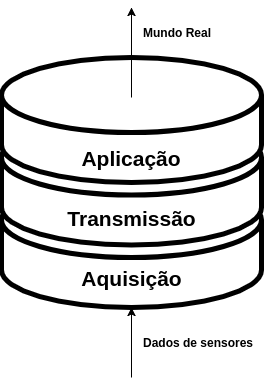
\includegraphics[width=5cm]{./02_Capitulos/02_Cap1/figures/iot_stack}
\caption{As três camadas do IoT, dos sensores ao mundo real}
\end{figure}

A primeira camada é a de aquisição de dados, que lida com o mundo físico e amostra estes dados através de sensores e conversores A/D, também realiza o processamento para entregar em um formato adequado para transmissão e entendível do outro lado, dependo da aplicação. A segunda camada é a camada de transmissão, onde estão, efetivamente, as camadas de rede embutidas. Como o nome já denuncia, ela lida com os aspectos de rede e comunicação para que o dados cheguem as seus destinos. E por último temos a camada de aplicação, a mais abrangente e que envolve maior poder computacional. Ela recebe os dados e lida com os processos de aplicação destes dados, seja análise, visualização, armazenamento ou a estruturação destes.

\subsection{Aquisição}
\label{subsection:aquisicao}

A etapa de aquisição está inserida diretamente no contexto de dados físicos, geralmente são hardwares menos complexos, focados em processamento de dados e entrada e saída com conversão analógico-digital. Se comunicam com sensores ou centrais de controle lógico. São responsáveis por:

\begin{itemize}
	\item Receber dados de sensores;
	\item conversão A/D;
	\item Processamento e calibragem de valores;
	\item Envio de dados em tempo real;
\end{itemize} 

Para atender essas tarefas, não é necessário grande poder de processamento, microcontroladores ou microprocessadores são capazes de atender tais necessidades se acompanhados de módulos de rede e portas I/O, assim como a implementação do software. Veremos dois exemplos no capítulo de implementação do projeto, que utilizam tanto MCU (Micro-Controller Units) ou Consoles com Sistemas Operacionais leves.
 

\subsection{Transmissão}
\label{subsection:transmicao}

Esta camada é o coração do IoT. A forma de transmissão define quais dispositivos eletrônicos e qual sua especificação técnica necessária para os quesitos de transmissão. Também define como os softwares da camada de aplicação e aquisição devem ser implementados baseado na estrutura da pilha de rede que será usada para transmitir.

Na próxima seção, veremos sobre a camada de rede e suas diversas formas de implementação. É importante que esta camada seja definida da melhor forma a atender sua aplicação, atendendo aspectos: 
\begin{itemize}
\item quantidade de dados transmitido;
\item número de acessos; 
\item distância entre dispositivos;
\item segurança;
\end{itemize}

\subsection{Aplicação}
\label{subsection:aplicacao}

A camada de aplicação encabeça a pilha do IoT. É ela que de fato trata os dados e realiza as aplicações deste. Ela disponibiliza os dados para o mundo real, podendo exercer múltiplas funções simultâneas incluindo:

\begin{itemize}
\item Armazenamento e Análise;
\item Visualização; 
\item Inteligência e aprendizado;
\item Serviços e servidores;
\item Gerenciamento e configuração;
\end{itemize}

Nesta camada estão presentes os endpoints apontados pela camada de aquisiçao, o destino dos dados. Bem assim como os servidores que gerenciam os clientes (geralmente implementados na camada de aquisição) e serviços e configurações oferecidos pelo sistema em si.

\section{Camadas de Rede}
\label{section:camadas_de_rede}

Como visto anteriormente, a camada de transmissão basicamente define a infraestrutura do sistema. Ela é construído com as camadas de rede como base. Portanto definir as camadas de rede e seus protocolos é definir a camada de transmissão em si.

Redes de computadores são complexas com diferentes aspectos a se preocupar. Dividir em camadas permite modularizar a implementação da rede, de modo que cada camada tenha uma tarefa na estrutura de comunicação dos aspectos físicos ao software. Como a camada de cima não precisa saber sobre os detalhes e especificações da camada de baixo, as mudanças de uma parte do sistema é transparente para o resto do sistema. Existem diversas formas de implementação de camadas, mas todas se baseiam em um modelo de referência, o modelo OSI \cite{Zimmermann:1988:ORM:59309.59310}.


\begin{figure}[h!]
\label{fig:1.2.0/modelo_osi_tcpip}
\centering
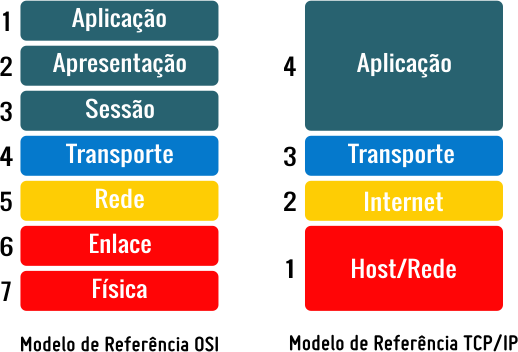
\includegraphics[width=8cm]{./02_Capitulos/02_Cap1/figures/modelo_osi_tcpip}
\caption{Diferenças entre OSI e TCP/IP em suas camadas}
\end{figure}

Baseado no modelo OSI. Temos o modelo TCP/IP \cite{TCPIP}, utilizado na internet e base para protocolos de aplicação muito utilizados como HTTP, WebSocket e MQTT. Em ambos cada camada exerce uma tarefa com seu respectivo protocolo, como resumido na tabela \ref{table:1.2.0}.

\begin{table}[h]
\centering
\caption{As camadas e e suas funções}
\begin{tabular}{|l|l|}
\hline
\multicolumn{1}{|c|}{CAMADA} & \multicolumn{1}{c|}{DETALHES}                                                  \\ \hline
7 - Aplicação                & Define instruções específicas da aplicação          						    \\ \hline
6 - Apresentação             & Formatação dos dados, conversão dos dados                     					\\ \hline
5 - Sessão                   & Negociação e conexão com outros nós, analogia                                \\ \hline
4 - Transporte               & Oferece métodos para a entrega de end-to-end                        			\\ \hline
3 - Rede                     & Roteamento de pacotes em uma ou várias redes                                 \\ \hline
2 - Enlace                   & Detecção de erros;                                                            \\ \hline
1 - Física                   & Aspectos físicos da transmissão \\ \hline
\end{tabular}
\label{table:1.2.0}
\end{table}


O foco desta literatura está na camada de aplicação e suas funcionalidades. Apesar de diferentes tecnologias utilizarem diferentes camadas abaixo, serão especificas características de protocolos construídos em cima do TCP/IP, por seu uso na Internet e redes industriais, e que sejam eficientes em trocas de mensagens em tempo real.


\chapter{A Interface e sua ligação com IoT}
\label{chapter:interface_iot}

No capítulo \ref{chapter:industria_4_0_iot}, foi visto as bases para se implementar um projeto de IoT. A área começou a receber fortes investimentos e atenção por volta de 2009 e desde então foram feitas consideráveis implementações utilizando tecnologias e protocolos diferentes. Neste capítulo serão apresentados algumas dessas variações, para fins de comparação e respaldo para importância e objetivo deste projeto.


\section{Algumas tecnologias em IoT}
\label{section:tecnologias_iot}

Estas são algumas tecnologias que satisfazem as condições apresentadas para um sistema IoT, nem todas utilizam o protocolo TCP/IP, mas todas são  capazes de fazer seus dispositivos comunicarem-se em tempo real levando em consideração seus alcances e escalabilidade.

\subsection{RFID}
\label{subsection:rfid}

As primeiras aplicações de IoT foram em laboratórios de aplicações de RFID \cite{Rampim:iot}, junto com códigos bidimensionais, para aplicações de identificação de objetos. Uma das soluções mais populares e de baixo custo de IoT utilizando Rádio frequência.

\subsection{Redes NB}
\label{subsection:nb}

Redes que utilizam bandas restritas visando baixo consumo e distância de transmissão são a nova fronteira, as mensagens de IoT são geralmente curtas, dados telemétricos, status etc, logo estes protocolos mostram-se úteis para este tipo de aplicação. Já se encontram implementadas algumas redes como SigFox \cite{Sigfox} e LoRa \cite{LoRa}. 

\subsection{Low Energy Bluetooth}
\label{subsection:bluetooth}

As novas gerações de Bluetooth consomem muito menos energia, o que tornaram a tecnologia viável para aplicações IoT. Geralmente, módulos Bluetooth são utilizados como beacons \cite{Endeavor:Beacons}. Pontos espalhados por uma região, no qual podem se comunicar com os módulos de dispositivos mobile ao se aproximar, oferecendo links para conteúdo e exclusividades.

\subsection{Base TCP/IP}
\label{subsection:tcpip}

As tecnologias mais comuns de se encontrar em aplicações IoT, os protocolos construídos com base no TCP/IP são vastamente utilizados e possuem uma rede mundialmente distribuída, o que facilita o uso. Pode-se implementar uma gama de protocolos de aplicações, alguns mais eficientes que outros.

O protocolo mais simples seria o HTTP, altamente usado na internet, porém não é eficiente no consumo de energia por abrir uma conexão a cada envio de dados. Para minimizar estas desvantagens, foi desenvolvido o CoAP \cite{coap} protocolo nos mesmos moldes do HTTP com o modelo REST, porém mais simples, mais leve, com baixo overhead e utilizado em redes locais.

Mas os mais utilizados em aplicações são sem dúvidas os protocolos que mantém conexão aberta, em especial Websocket e MQTT, sendo o primeiro mais utilizado para chats e mensagens e o segundo domina o mundo do M2M e Telemetria.


\section{A Interface}
\label{section:interface}

Inicialmente, os conceitos e ideias do projeto eram voltados a desenvolver uma interface no qual um desenvolvedor poderia implementar um sistema IoT de ponta a ponta utilizando APIs que direcionariam para um desses protocolos da seção \ref{section:tecnologias_iot}, porém as diferenças entre os protocolos e as camadas de base, fazem com que esta solução esteja mais distante. Então o foco voltou-se  para tecnologias que tenham base na pilha TCP/IP, por sua vasta implementação nas redes industriais e residências e na Internet.

Neste projeto iremos ver a implementação desta interface para o protocolo MQTT, cuja escolha será justificada adiante. Serão descritas as interfaces para as três camadas, que são de baixo custo, open-source e altamente escaláveis para construir outras aplicações com esta como base.
 
Para abstrair as camadas e aplicação, a interface deve estar dentro dos requisitos do IoT, bem assim como apresentar uma estrutura que se traduza aos protocolos baseados TCP/IP, para isso, algumas características fundamentais podem ser destacadas como base para um sistema IoT descritos.

\begin{itemize}

\item Full-Duplex. Capaz de receber e enviar mensagens ao mesmo tempo;
\item Multicast. Capaz de enviar mensagens um ou mais dispositivos simultâneos;
\item Envio de mensagens em tempo real;

\end{itemize}


\begin{figure}[h!]
\label{fig:2.2.0/camada_abatracao}
\centering
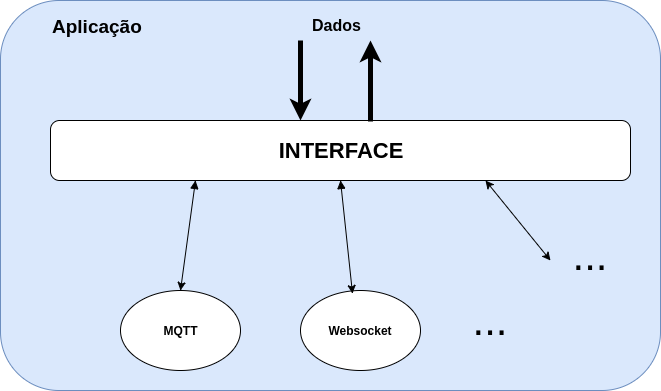
\includegraphics[width=12cm]{./02_Capitulos/02_Cap2/figures/camada_abstracao}
\caption{Interface de comunicação. A interface tem seu próprio protocolo que direciona e se comunica a um ou mais protocolos de aplicação}
\end{figure}

Essas características estão dentro do escopo apresentado no capítulo \ref{chapter:industria_4_0_iot}, a estratégia foi direcionada para protocolos que atendessem esse pré-requisito, assim construindo uma camada de abstração da interface por cima dos protocolos que contemplam essas características como mostra a figure \ref{fig:2.2.0/camada_abatracao}, o que será mais detalhado no próximo capítulo.



\chapter{O Projeto}
\label{chapter:projeto}

Os dois últimos capítulos descreveram o conceito de Internet das Coisas e as especificações que o projeto deve contemplar, visando sempre ajudar na construção de sistemas IoT que melhor se encaixem na aplicação. Neste capítulo serão descritos as implementações do projeto, apresentado os motivos das escolhas de tecnologias e protocolos especificados. E terminando sobre persistência de dados em aplicações IoT e por quê a escolha de implementação bancos de dados é importante para a aplicação.


\section{Camada de Abstração}
\label{section:camada_abstracao}

Devido a interação entre dispositivos de aquisição de dados e aplicação e armazenamento de dados, foi necessário uma implementação de um protocolo de comunicação único entre os dispositivos e implementação em cada um destes em suas diferentes linguagens de programação.

O protocolo consiste em uma abstração de um canal de envio de dados chamado Data Stream mostra
do em \ref{fig:3.1.0/data_stream}, no qual passam dados após realizar um processamento dos dados em uma determinada velocidade podendo conter um limite de pacote de dados. Nas pontas desse canal estão os Publishers e Subscribers, que serão descritos adiante. Este conceito é uma forma de abstrair, unificar e simplificar a forma de transporte de dados, de uma modo que a interface possa ter o controle sobre os aspectos de transmissão. Cada protocolo na camada de aplicação, implementa este conceito de uma certa forma, porém o desenvolvedor não precisará se preocupar com estes detalhes.

\begin{figure}[h!]
\centering
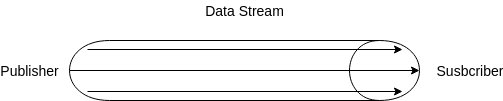
\includegraphics[width=13cm]{./02_Capitulos/02_Cap3/figures/data_stream}
\caption{O conceito de Data Stream para a abstração do transporte de dados}
\label{fig:3.1.0/data_stream}
\end{figure}


\section{Publishers e Subscribers}
\label{section:publishers_subscribers}

Para enviar e receber dados de uma forma a atender os requisitos da seção \ref{section:interface}, foi utilizado um padrão de comunicação recorrente em aplicações contemporâneas, o padrão Publish/Subscribe \cite{amazon:pub-sub}.

O padrão Publish/Subscribe permite que as mensagens sejam transmitidas assíncronas e para vários dispositivos simultaneamente. Para transmitir uma mensagem, um client pode simplesmente enviar uma mensagem para o tópico que os envia imediatamente para todos os subscribers. Todos os componentes que se inscreverem no tópico receberão todas as mensagens transmitidas, a menos que uma política de filtragem de mensagens seja definida pelo assinante.

\begin{figure}[h!]
\centering
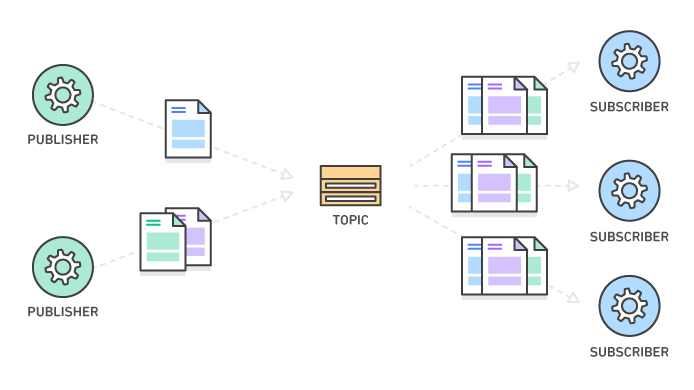
\includegraphics[width=12cm]{./02_Capitulos/02_Cap3/figures/aws_pub_sub}
\caption{O padrão Publish/Subscribe. Retirado de \cite{amazon:pub-sub}}
\label{fig:3.2.0/aws_pub_sub}
\end{figure}

Qualquer mensagem publicada em um tópico é imediatamente recebida por todos os subscribers do tópico. As mensagens de podem ser usadas para arquiteturas orientadas a eventos ou para desacoplar aplicativos, aumentando  o desempenho, a confiabilidade e a escalabilidade. Com isso, foram criados duas funções possíveis para cada dispositivo dentro deste padrão, os Publishers e os Subscribers, sua comunicação é descrita em \ref{fig:3.2.0/pub_sub}.




Publishers são dispositivos que criam Data Stream  e enviam dados por estes, regulam o processamento dos dados estipulam limites de tamanho de cada pacote de dado e determinam o intervalo de envio de pacotes. O protocolo permite que estes enviem os dados e também permite que outros dispositivos possam passar configurações remotamente para modificar os parâmetros de cada Data Stream, como o intervalo de envio ou outra configuração criada pelo tipo de Data Stream implementado. 


\begin{figure}[h!]
\centering
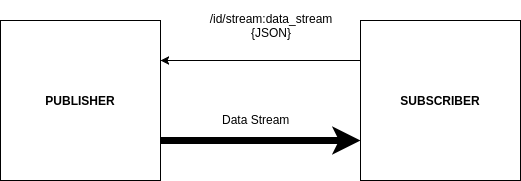
\includegraphics[width=12cm]{./02_Capitulos/02_Cap3/figures/publisher-subscriber_comm}
\caption{Comunicação entre Publishers e Subscribers por Data Stream}
\label{fig:3.2.0/pub_sub}
\end{figure}

Subscribers estão na outra ponta recebendo os dados, são capazes de enviar as configurações do Data Stream para os Publishers a chegada destes dados como um driver para a aplicação
Essas funcionalidades foram implementadas Orientadas a Objeto e são escaláveis para aplicações mais complexas que serão implementadas para o uso dos sistemas em aplicações de sensoriamento e visualização dos dados.

\section{A implementação}
\label{section:implementacao}

%%% MQTT , Websocket e HTTP %%%
Existem protocolos de aplicação que podem ser facilmente mapeados por esse tipo de interface. Alguns já são cosntruídos no modelo Publish/Subscribe, outros em modelos parecidos. Para critérios de comparação, apresentam-se dois protocolos de aplicação, MQTT e WebSockets \cite{websocket}. O protocolo MQTT, no qual será implementado nesse projeto, foi moldado no padrão citado, enquanto o WebSockets é orientado a eventos. Ambos enviam mensagens em tempo real através de um servidor que controla o fluxo de mensagens da aplicação.

Na questão de desempenho, estes protocolos se mostram mais eficientes dentre os construídos sobre TCP/IP, comparado, por exemplo, com o HTTP, protocolo de rede mais recorrente em redes locais e na internet. Como mostrado em \cite{Tetsuya-Sasaki} e \cite{Naik}, HTTP, por sua natureza de abrir e fechar conexão a cada requisição de dados e seu cabeçalho, requer mais banda e consome mais energia que protocolos leves e de conexão persistente como os dois acima. O que faz sua escolha remota para a aplicação deste projeto.


\subsection{MQTT}
\label{subsection:mqtt}

O protocolo MQTT \cite{mqtt} foi utilizado escolhido por ser leve e ideal para aplicações em tempo real com vários dispositivos simultaneamente. É um protocolo no padrão Publish/Subscribe  ideal para definir a função de cada dispositivo seja enviando dados (Publish) ou recebendo estes (Subscribe).

Para gerenciar os clients (responsáveis pela implementação da comunicação MQTT) em cada dispositivo é necessário um servidor chamado Broker. Este foi implementado com o Mosquitto \cite{mosquitto}, um broker open source e leve capaz de ser instalado localmente e no servidor do laboratório para testes remotos.

\subsubsection{Broker}
\label{subsubsection:broker}

O Broker é o servidor do padrão Publish/Subscribe, ele efetivamente executa as ordens de publicação (publish) feita por algum cliente para os tópicos que outros clientes estão inscritos (subscribed), possui todas as listas de tópicos, é orientado a conexão e não persiste informações dos clientes, ou seja, em caso de queda de conexão, estes devem se inscrever novamente nos tópicos.

\textit{Nota: A arquitetura Broker não é exclusividade do MQTT, outros protocolos utilizam esse tipo de implementação em servidores.}


\begin{figure}[h]
\centering
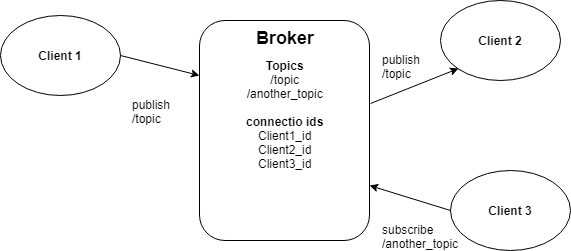
\includegraphics[width=12cm]{./02_Capitulos/02_Cap3/figures/broker_pub_sub}
\caption{Exemplo de gerênciamento de um broker}
\label{fig:3.2.0/broker_pub_sub}
\end{figure}

Na figura \ref{fig:3.2.0/broker_pub_sub}, o Broker armazena os tópicos e os ids de conexão dos clientes, 2 estava inscrito para ouvir as mensagens do tópico \textit{topic}, enquanto 3 enviava uma ordem de inscrição em \textit{another\_topic}, 1 envia ordem de publicação para \textit{topic}.


\subsection{Tipos de MQTT}
\label{subsection:tipos_mqtt}

%% Tipos de MQTT 
Com a evolução e o uso do protocolo, foram necessárias atualizações que contemplam funcionalidades que atendem  requisitos essenciais para aplicações da indústria. Como atender dispositivos que não usam a pilha TCP/IP e medidas de segurança (que serão melhor debatidas á frente). 

\subsubsection{MQTT-SN}
\label{subsubsection:mqtt-v}

Existe uma gama de dispositivos que utilizam protocolos específicos, geralmente leves, para redes locais e leves para o transporte de dado, a exemplo do ZigBee \cite{zigbee}. Para isso foi criada uma versão do MQTT para atender estes tipos de protocolos, substituindo a base TCP/IP por outros protocolos destas camadas, mantendo a camada de aplicação e o padrão Publish/Subscribe.

\subsubsection{MQTTS}
\label{subsubsection:mqtts}

Para resolver questões de segurança, foi criada uma variação do MQTT que adiciona camadas deste quesito ao protocolo de aplicação. Assim como o HTTPS o protocolo MQTTS é construído em cima do protocolo SSL/TLS (explicado em \ref{subsection:seguranca}), camada de segurança que também usa como base TCP/IP. Esta camada envolve o processo de encriptação dos cabeçalhos da aplicação e autenticação por passagem de certificados. 

\subsection{Segurança de aplicações}
\label{subsection:seguranca}

%% SSL e outros tipos de encriptação de dados.
SSL \cite{ssl} (Secure Sockets Layer) é a tecnologia de segurança padrão para estabelecer um link criptografado entre um servidor da Web e um cliente. Um certificado SSL em seu servidor e um navegador se conecta a ele, a presença do certificado SSL aciona o protocolo SSL (ou TLS), que criptografa as informações enviadas entre o servidor e cliente.

O SSL opera diretamente no topo do protocolo de controle de transmissão (TCP), além de permitir que camadas de protocolo de aplicaçãoes sejam construídas por cima, agora com sob uma camada de segurança. Portanto, sob a camada SSL, as outras camadas de protocolo podem funcionar normalmente, como o HTTP e o MQTT.

Com um certificado SSL, todos os invasores poderão saber qual IP e porta e quantos dados estão sendo enviados. Eles podem terminar a conexão, mas tanto o servidor quanto o usuário poderão dizer que isso foi feito por terceiros. No entanto, eles não serão capazes de interceptar qualquer informação, o que a torna essencialmente um passo ineficaz. O invasor pode descobrir qual nome de host,mas como a conexão é criptografada, as informações importantes permanecem seguras.

Para poder criar uma conexão é requisitado um Certificado SSL. Quando você optar por ativar o SSL em seu servidor da Web, será solicitado que você responda a várias perguntas sobre a identidade do seu site e da sua empresa. Seu servidor da Web cria duas chaves criptográficas - uma chave privada e uma chave pública.

A chave pública não precisa ser secreta e é colocada em uma solicitação de assinatura de certificado (CSR) - um arquivo de dados que também contém seus detalhes, então deve-se enviar o CSR. Durante o processo de solicitação do Certificado SSL, a Autoridade de Certificação validará seus detalhes e emitirá um Certificado SSL contendo seus detalhes e permitindo que você use SSL.

Além do SSL existem outras formas de segurança. A maioria envolve encriptação. Como o uso de algoritmos de hash para encriptar as mensagens enviadas, ficando a cargo da aplicação desencriptar.

\subsection{Plataformas}
\label{subsection:plataformas}

%% ESP e Raspberry
Para que o sistema esteja completo, é necessário estender a interface a camada de aquisição e aplicação da pilha do IoT, para isso, foi necessário criar SDKs (Software Development Kits) para plataformas que suportem o protocolo TCP/IP. E que possam ser utilizadas em sistemas IoT. Para a camada de aplicação, foram focados em plataformas embarcadas com acesso a rede e para a aplicação, plataformas com sistemas operacionais, podendo suportar aplicações mais complexas.

A camada de aquisição apresenta implementação dos Publishers, pois são que enviam os dados, as plataformas possuem unidades de processamento e módulos de rede o que as torna ideais para publishers, porém não tão eficientes para serem Subscribers. Estes últimos são implementados na camada de aplicação, onde estão dispositivos com maiores recursos e com a função de receber dados e criar aplicações em cima desta função básica.

\subsubsection{Embarcados}
\label{subsubsection:embarcados}

Embarcados, são sistemas alimentados por baterias, sem alimentação de rede elétrica, portáveis, econômicos, com sistemas de controles geralmente feitos por microcontroladores ou microprocessadores, podendo contemplar sistemas operacionais leves. Com essa descrição, pode-se imaginar que estes dispositivos possuem processamento, energia e desempenho limitados. Para isso foi necessário a criação de uma implementação de interface leve e eficiente

Foi escolhida as plataformas microcontroladas pela arquitetura Espressif \cite{espressif}. MCUs(Micro-Controller Units) que contemplam processadores e módulos WiFi e até Bluetooth (não utilizado na interface atual), mostrados em \ref{fig:3.3.4/esp32-arch} na arquitetura do esp32, pela descrição técnica pode-se ver um poder de processamento maior que um Arduino \cite{arduino}, muito utilizado nessas aplicações e que também é compatível com a interface se adicionado shields WiFi. O ESP utiliza linguagem C++ \cite{c++} para desenvolvimento do Publisher e Data Stream, com framework Arduino que permite implementação em outras plataformas, além de uma firmware escalável, circuito open hardware e open source.

\begin{figure}[h!]
\centering
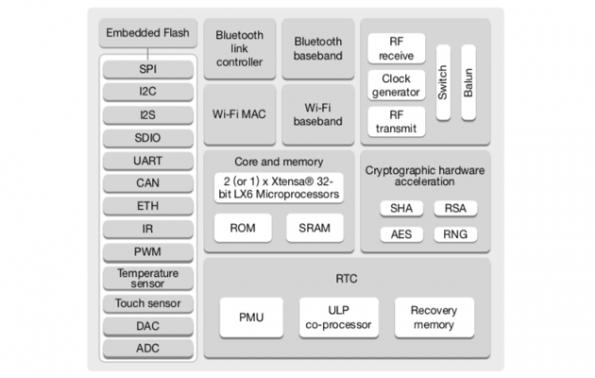
\includegraphics[width=13cm]{./02_Capitulos/02_Cap3/figures/espressif32-arch}
\caption{A arquitetura do ESP32, retirado de \cite{espressif}}
\label{fig:3.3.4/esp32-arch}
\end{figure}


Também foi implementada em Node.js (que será descrito abaixo) aplicações do Publisher para embarcados com sistemas operacionais baseados na arquitetura ARM \cite{arm}, como Raspberry Pi \cite{raspberry-pi} e sua arquitetura mais robusta \ref{fig:3.3.4/raspberry-pi-arch} , e Intel Galileo. Permitindo multi-uso entre as funções de Publisher e Subscriber, podendo ser utilizados como Hubs ou bridges de dados. Esses consoles possuem, processadores mais potentes, periféricos, Sistemas Operacionais, assim como entradas e saídas digitais.

\begin{figure}[h!]
\centering
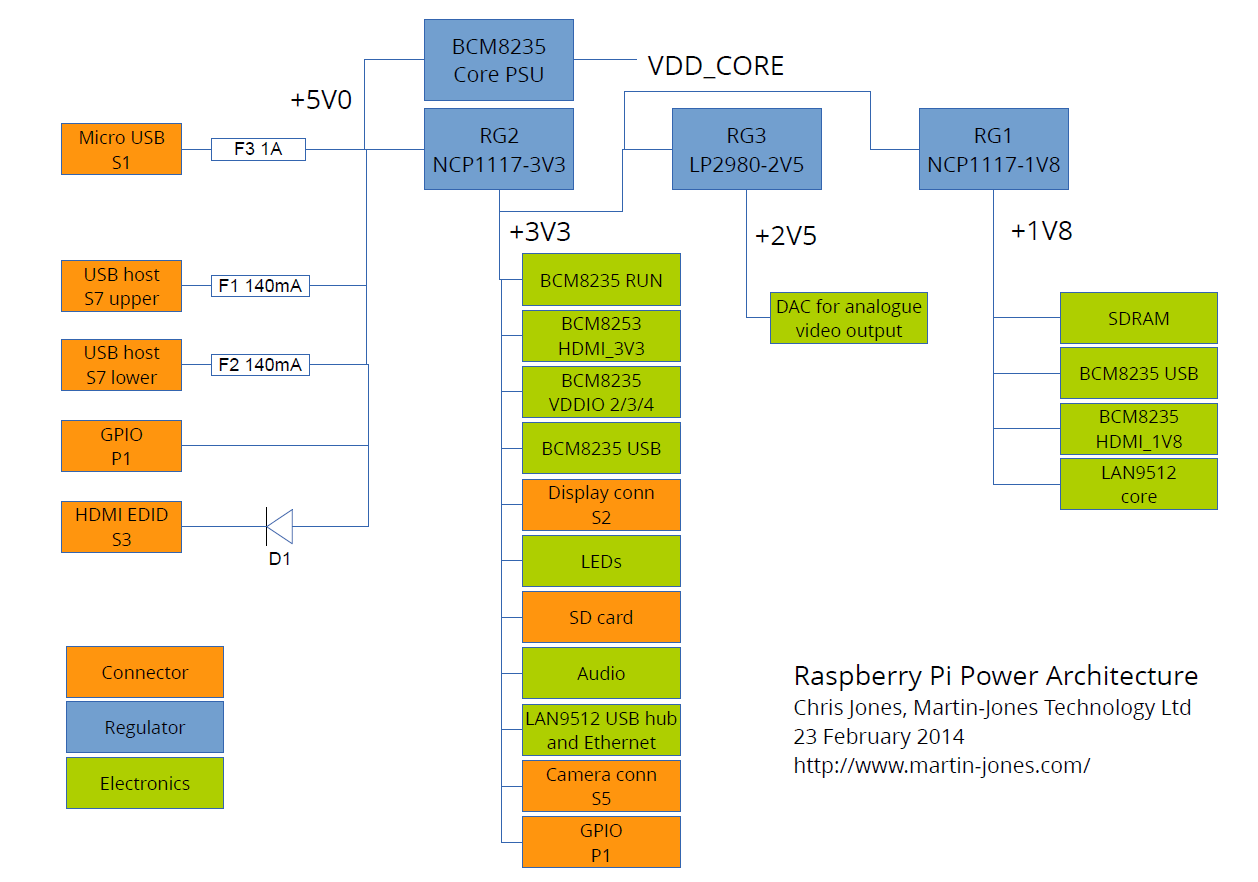
\includegraphics[width=13cm]{./02_Capitulos/02_Cap3/figures/raspberry-pi-power-architecture}
\caption{A arquitetura do micro console Raspberry-Pi}
\label{fig:3.3.4/raspberry-pi-arch}
\end{figure}

\subsubsection{Consoles}
\label{subsubsection:consoles}

Consoles são sistemas que contemplam sistemas operacionais, o que permitem mais liberdade para a implementação da interface. Foi escolhida então, realizar a implementação com Node.js \cite{nodejs}, uma engine de Javascript que permite criar aplicações no lado do servidor de um sistema, além de outras aplicações, como mobile e desktop. Possui extensas bibliotecas para HTTP e MQTT além de pipelines que permitem fácil comunicação de protocolos no mesmo processo, o que é fundamental para o conceito de escalabilidade deste projeto.

Além disso Node.js é uma ferramenta multiplataforma, com distribuições para Windows, Linux e MAC, além de versões para embarcados de arquitetura ARM, como o próprio Raspberry Pi. Com isso foram implementadas bibliotecas que constroem e interface sobre o MQTT, no lado Subscriber do sistema.

\subsection{Persistência de dados}
\label{subsection:persistencia}

%% Bancos de dados
Os dados adquiridos pela plataforma e suas camadas, são armazenados em memórias e enviados. Memórias voláteis que podem facilmente perder dados com quedas de energia o reaproveitamento do sobre-inscrição do próprio gerenciamento do sistemas, para garantir que os dados não sejam perdidos, é necessário que o sistema possua persistência, uma forma de memória não-volátil que armazene os dados sem energia.

Essa persistência é implementada com Banco de Dados, estruturas que organizam o armazenamento de dados persistentes em arquivos. Um Banco de dados é uma basicamente uma aplicação, um serviço do sistema que recebe requisições de rede e escreve ou lê dados em um arquivo. Existem inúmeras formas de implementação e protocolos de comunicação para Bancos de Dados. Porém todos eles seguem abstrações em comum.

Um banco é composto por duas ferramentas. O Motor e o Arquivo de dados. O motor é quem realiza as ações sobre o arquivo, é o sistema de gerenciamento. Recebe as requisições e aplica algoritmos de escrita de dados eficientes no arquivo para armazenar os dados em uma estrutura definida. Um Banco de dados pode possuir vários motores, cada um com algum algoritmo que varia a eficiência e o tempo de escrita e/ou leitura dependendo do dado recebido.

\begin{figure}[h!]
\centering
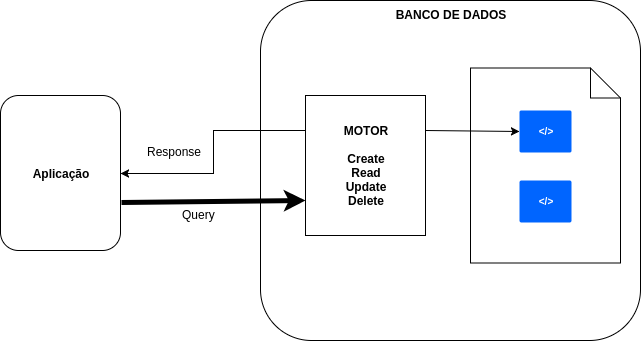
\includegraphics[width=12cm]{./02_Capitulos/02_Cap3/figures/Database_Arch}
\caption{A arquitetura de um banco de dados}
\label{fig:3.3.5/database_arch}
\end{figure}

O Arquivo é o documento onde os dados são armazenados, na estrutura definida. Possuem formatações de dados específicas de cada tipo de banco, seguindo uma abstração. O formato do armazenamento de dados, define e limita eficiência do motor, então e necessário a escolha adequada de algoritmo para uma maior eficiência da leitura do arquivo. Como em \ref{fig:3.3.5/database_arch} a aplicação envia uma solicitação de criação ou leitura ou atualização ou remoção (CRUD - Create, Read, Update, Delete) e o motor lida com os dados, armazenando-os em uma determinada estrutura no Arquivo.


 
\subsection{Bancos para Aplicações IoT}
\label{subsection:bancos_IoT}

Na área de Bancos de Dados (ou DBs), com escopo focado em IoT, há um porém. Para a estruturação de uma aplicação eficiente, não se deve usar qualquer tipo de banco. Devem-se escolher motores e estruturas de bancos adequadas para a aplicação. Não exite um critério definitivo que guia o desenvolvedor para melhor escolha. Mas algumas características de bancos de dados podem ser exploradas em aplicações IoT, formando um DB eficiente para tal.

Como pode ser observado em \cite{Damodaran}, uma aplicação eficiente de Bancos e IoT está ligada ao tempo de inserção de dados no banco,  o tempo total em que a aplicação leva para enviar, aplicar a busca de onde o dado deve ser inserido no documento e de fato armazenar, podem ser feitas várias inserções de pequenos pacotes de dados, dependendo do tamanho da mensagem. Esta característica está ligada ao motor do banco, que determina como o dado será armazenado, e quanto ele leva para escrever o dado no documento. A maioria dos dados são armazenados em estruturas B+- Trees , porém pode-se observar em \cite{Damodaram} e \cite{oneal} que a estrutura LSM Tree, feita através da B+-, possui maior eficiência na escrita.

Existem várias abstrações de Bancos de dados. Em \cite{Rautmare-Bhalerao} compara-se e conclui-se que o banco MongoDB, um banco NoSQL possui um tempo de resposta de inserção menor que o MySQL (bancos relacionais), porém o último é mais estável. De fato bancos NoSQL são, em geral, mais leves, possui uma flexibilidade maior para lidar e estruturar dados, o que fazem estes tipos de Banco mais favoráveis a aplicações de IoT. Porém outras estruturas como um banco divido em timescale mostram-se eficientes SQL ou não.

Outros aspectos podem contribuir para a eficiência de persistência de dados. Criar bancos locais diminuem a latência e a necessecidade de conexão, aumentando a capacidade de inserção de dados, além de ser uma forma de backup de dados. Um banco local, geralmente fica em uma plataforma como em \cite{Paethong-Sato-Namiki}, são bancos leves em aplicações de baixo consumo, devido a capacidade de processamento limitada. Seu papel é geralmente para armazenar os dados quando não há conexão, e quando esta é restabelecida os dados são enviados para um banco remoto com mais capacidade de processamento e aplicações. %% Falar sobre bancos locais.

Dentre os bancos estudados, alguns se destacam como o Cassandra, usado pela Netflix para coletar dados sobre o comportamento do usuário na plataforma ou o InfluxDB, um banco de arquitetura TimeScale, feito para aplicações em tempo real. Mas para esse projeto, foi utilizado o MongoDB \cite{mongodb}, um banco NoSQL, leve, de facil integração com as plataformas utilizadas e que posui implementações de motores que priorizam a eficiência na escrita de dados, como a LSM tree.
\chapter{Casos de Uso}
\label{chapter:casos_de_uso}

% Escrever sobre caso de uso do sistemas
No capítulo \ref{chapter:projeto} descrevemos o funcionamento da Interface e sua comunicação com a linguagem MQTT. Este capítulo busca demonstrar o funcionamento do sistema em hardwares com a interface implementada pelos softwares descritos na seção \ref{section:codigos_fonte} disponível no Apêndice. São aplicações simples que mostram a facilidade e a escalabilidade do sistema, além de demonstrar como o sistema pode ser implementado em plataformas.

\section{Medição de temperaturas de CPU}
\label{section:temp_cpu}

\textbf{obs:} \textit{Para reproduzir este teste, é necessário seguir as instruções encontradas no Apêndice}.

Este exemplo tem como objetivo medir a temperatura da CPU de um console com baseado em suas atividades, serviços e processos em execução. A aplicação pode ser escalada para a obtenção de outras informações da CPU e do sistema, podendo assim disponibilizar análises de desempenho da plataforma, além de montar perfis de uso do sistema e administrar seu uso.

A escalabilidade do sistema será testada em partes, a primeira será analisar medições de temperatura de uma CPU de um console. Em seguida comparar medições de temperatura da CPU com um ESP32 e por último analisar temperatura de múltiplas CPUs.

Para isso precisaremos utilizar uma instância da classe Publisher disponível  \ref{subsection:publishers_javascript} como e no console a ter informações de temperatura a ser coletadas e uma instãncia do Subscriber \ref{subsection:subscribers_javascript} para receber estas temperaturas via MQTT e persisti-las em banco de dados. Ambas as aplicações utilizarão as APIs em Javascript, utilizando Node.js para coletar as informações do sistema, implementar o Publisher, o Subscriber, o driver para MongoDB (também disponível em anexo) e a geração de um gráfico utilizando a plataforma plotly \cite{plotly}. Isso foi implementado no código \ref{subsection:teste_fonte}.

CPUs são tecnologias feitas por transistores. Milhões de aglomerações de MOSFETS que começam a  ter perda de perfomance no processador conforme o aumento de temperatura, em \cite{jose}, pode-se observar os efeitos do aumento de  temperatura nos parâmetros do MOSFET especialmente na queda de mobilidade e na velocidade de saturação que provocam perda de perfomance. CPUs modernas são capazes de ajustar suas frequências operacionais, a fim de reduzir seu consumo de energia ou fornecer a máxima potência, conforme necessário e possuem também  proteção térmica extremamente robusta. Se a unidade começar a operar acima do limite térmico, ela começará a reduzir a frequência para evitar uma falha catastrófica.

\begin{figure}[h!]
\centering
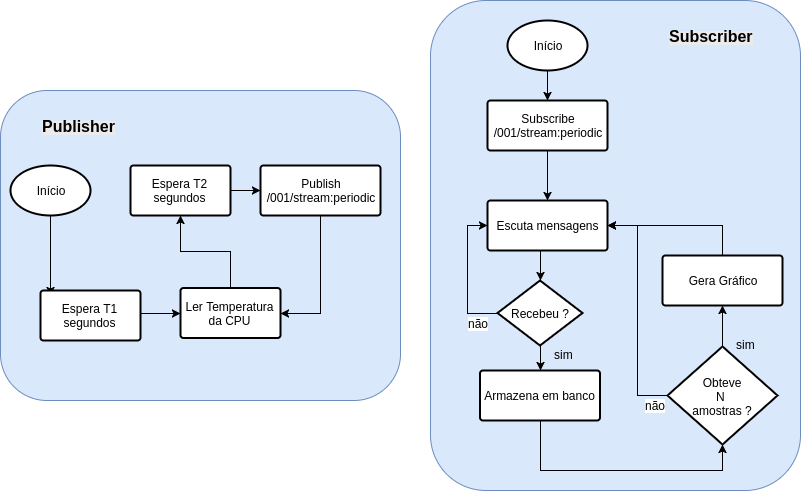
\includegraphics[width=11.5cm]{./02_Capitulos/02_Cap4/figures/fluxo_controle_temp}
\caption{Diagrama de fluxos do Publisher e do Subscriber}
\label{fig:4.1.0/fluxo_controle_temp}
\end{figure}

% Falar sobre o diagrama de fluxo
A \ref{fig:4.1.0/fluxo_controle_temp} mostra todo o fluxo das duas aplicações, o Publisher publica em no tópico \textit{/001/stream:periodic}, a informação coletada a cada T1=3 segundos e espera T2=1 antes de enviar. O Subscriber escuta este tópico e persiste ao chegar uma mensagem de dados pelo Data Stream, ao atingir N=100 amostras, um gráfico de Temperatura da CPU principal pela Data-Hora de inserção é gerado com as últimas 100 inserções no banco.


% Inserção no banco
Repare que a medição depende da data e da hora de inserção no banco, o tempo de chegada até a persistência varia muito com a latência e com o processamento da aplicação, desta forma temos uma medida mais constante. A \ref{fig:4.1.0/compass} mostra o formato de dado armazenado, com a ferramenta Compass para visualização de dados do MongoDB. Repare que lidamos com a estrutura de dados em documento porém obrigatoriamente todo documento da Interface possui o timestamp da inserção no banco, o campo data é o objeto de dados em medição. A comunicação com o banco pode ser feita por uma instância da classe MongoDataClient em   \ref{subsection:subscribers_javascript} que cuida da inserção com  o \textit{timestamp} e o objeto de dados em \textit{data}.

\begin{figure}[h!]
\centering
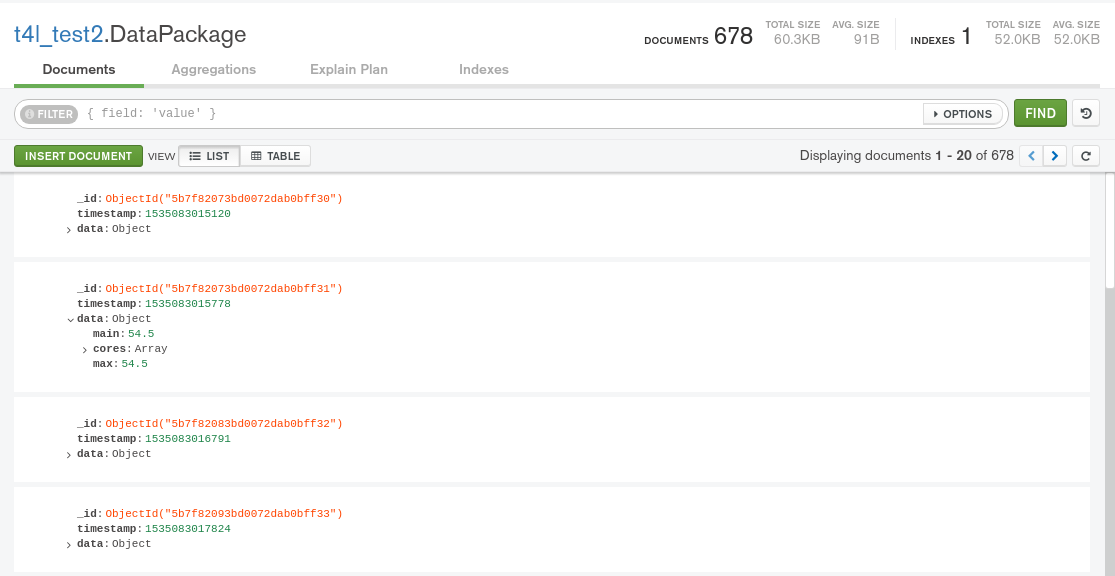
\includegraphics[width=15cm]{./02_Capitulos/02_Cap4/figures/compass}
\caption{Visualização dos dados armazenados em documento em uma coleção do MongoDB}
\label{fig:4.1.0/compass}
\end{figure}

% Visualização com o plotly
A visualização de dados é feita pela ferramenta Plotly, um serviço que fornece uma interface para criar, editar e analisar gráficos, basta criar uma conta, gratuíta ou paga, e o usuário poderá criar gráficos na plataforma web ou através de APIs implementadas em múltiplas linguagens de programação conhecidas. A aplicação do Subscriber utiliza da segunda opção com o módulo plotly.js, a implementação em Javascript da plataforma. A cada N=100 amostras são produzidos gráficos como o da  \ref{fig:4.1.0/cpu-temp_1}.


\begin{figure}[h!]
\centering
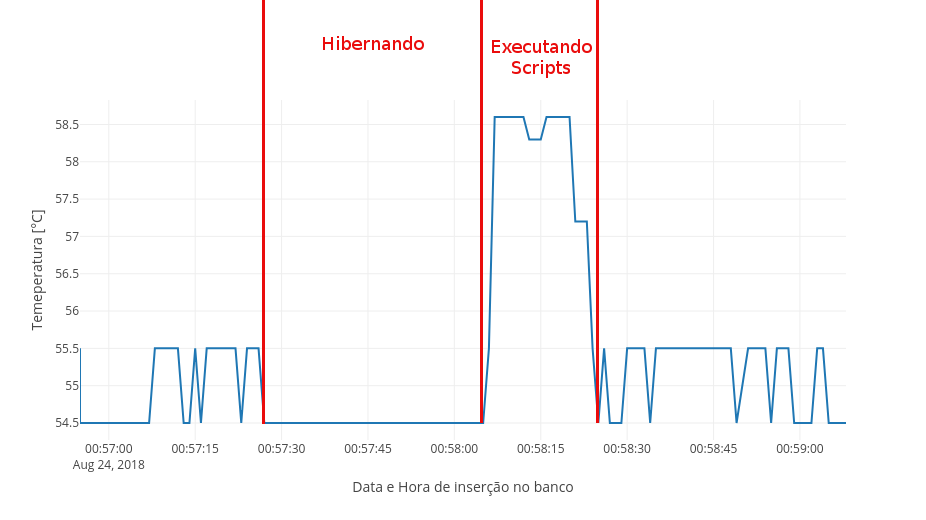
\includegraphics[width=16cm]{./02_Capitulos/02_Cap4/figures/cpu-temp_1}
\caption{Comportamento da temperatura em três momentos}
\label{fig:4.1.0/cpu-temp_1}
\end{figure}

A \ref{fig:4.1.0/cpu-temp_1} mostra a variação da temperatura de uma CPU da Intel Core I7 em três momentos. O gráfico começa no primero momento onde só os processos básicos do computador estão em execução, mantendo a temperatura constante, logo em seguida entra o momento onde o computador está hibernando o que leva a uma pequena baixa na temperatura. O terceiro momento descreve o comportamento quando o computador executa o MATLAB em um script que exige capacidade de processamento, causando uma leve alta de temperatura, mas não tão lata devido a capacidade do processador e depois estabilizando e voltando ao primeiro momento. Com isso fechando o ciclo das aplicações.


Finalizada a medição de uma CPU, pode-se escalar para uma Análise mais elaborada, junto as medições desta CPU core i7, foi acrescentada uma aplicação contendo um Publisher em um ESP32. Conforme descrito no capítulo anterior na \ref{fig:3.3.4/esp32-arch}, o ESP32 é um MCU que possui módulos WiFi e sensor de temperatura interno, facilitando a medição, como trata-se de um Microcontrolador foi utilizado a implentação em C++ \ref{subsection:teste-plataformas}, uma implementação síncrona.


\begin{figure}[h!]
\centering
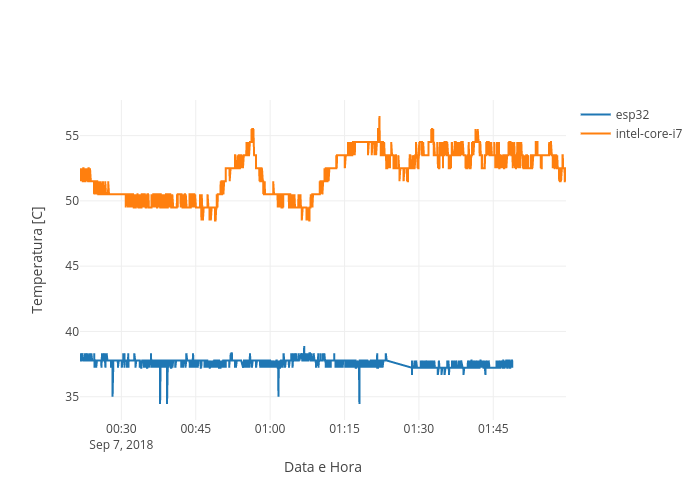
\includegraphics[width=16cm]{./02_Capitulos/02_Cap4/figures/temp-device-3}
\caption{Comparação das temperaturas com uma CPU core i7 e ESP32}
\label{fig:temp-devices-3}
\end{figure}

Ambas as plataformas foram configuradas para enviar informações de temperatura com intervalos de um segundo, durante um período de cerca de uma hora e meia, ao completar 10 mil amostras totais, um gráfico é gerado. Cada plataforma contribui com cerca de metade das amostras, porém cada uma possui uma rotina e capacidade de processamento, fora o tempo de envio para Broker, é de se esperar que o número de amostras de cada um não seja igual.
Pela \ref{fig:temp-devices-3} pode-se observar as diferenças de temperatura e o comportamento das duas CPUS. O ESP32 com sua arquitetura mais simples, mantem-se relativamente constante a 30 graus Celsius,  isso pode ser explicado devido ao fato do ESP estar rodando somente um programa devido suas limitações.
A CPU i7 varia sua temperatura em torno de 50 graus Celsius, possuindo variações mais bruscas, devido ao fato do processador está executando múltiplo processos. Durante este experimento o computado da CPU foi usado normalmente, passando por cenários de hibernação até o uso do Browser, recebendo requisições de páginas da web, assistindo vídeos e áudios, provocando as variações de temperatura semelhantes ao primeiro teste.


Por último o sistema foi utilizado em um teste em múltiplos computadores com processadores distintos no Laboratório PROSAICO. A finalidade foi observar o comportamento e a robustês da aplicação ao receber dados de múltiplas fontes em larga escala (cerca de 15 mil amostras totais no banco).

\begin{figure}[h!]
\centering
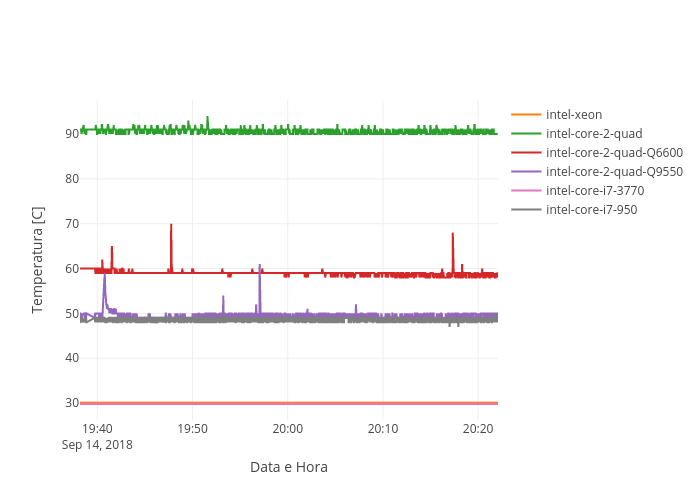
\includegraphics[width=16cm]{./02_Capitulos/02_Cap4/figures/temp-devices-5}
\caption{Comparação das temperaturas em múltiplos processandores}
\label{fig:temp-devices-5}
\end{figure}

Na \ref{fig:temp-devices-5}, observa-se vários níveis de temperatura média entre os processadores, todos executando processos comuns dos sistemas operacionais em máquinas Windows e Linux. Esta diferença está atrelada aos fatores de resfriagem térmica e a capacidade de processamento. Vale ressaltar alguns comportamentos. Os dois processadores de temperatura mais baixa, por volta de 30 graus célsius possuem gabinetes mais novos e apresentam um sistema de resfriamento melhor que os mais antigos. Já o processador que registrou uma maior temperatura média, fora o processador do computador usado como servidor Web e IoT do laboratório, hospedando o Broker Mosquitto do sistema, inclusive. Dois fatores contribuiram para essa mudança abrupta de tecnologia, os processos executados dos serviços, porém majoritariamente pela manuntenção do resfriamento do processador, foi detectado que a CPU estava sem pasta térmica, grande responsável pela troca de calor na prórpia.


\section{Aplicação: Automação Residencial}
\label{section:residencial}

Para validar o baixo custo do sistema, as próximas seções tem o foco em simular o orçamento de dois projetos. Um feito para a indústria e outro em redes domésticas para automações residenciais. Serão propostos cenários de aplicações reais, capazes de confirmar a premissa do projeto.
Como vimos no capítulo de projetos, o sistema pode ser instalado em plataformas mais sofisticadas, contendo sistemas operacionais e hardware dedicado. Mas nestes cenários utilizaremos o hardware mínimo que é compatível com o sistema e atua satisfatoriamente na aplicação.


O caso em estudo é a automação parcial de uma residência. Como pode ser visto em  \ref{fig:5.1.0/planta-casa}, a casa possui dois quartos, sala de estar, dois banheiros, cozinha, área de serviço e varanda. O objetivo é monitorar a temperatura local, o consumo de energia, detectar aberturas de portas e janelas de entrada da residência para fins de segurança e acionamento de luzes.

Para isso é necessário acionadores para a sala e cozinha, mais os quartos, totalizando cerca de 4 pontos de luz para acionar, o mesmo vale para os sensores de temperatura, no qual farão a média de temperatura da casa. Para controle de consumo de energia, nos limitaremos as tomadas de eletrodomésticos e eletrônicos, que representam a maior parte do consumo, para um ponto na sala, nos quartos, na tomada da geladeira, micro-ondas e lavadora, cerca de 6 tomadas a colocar sensores de tensão e corrente AC para cálculo da potência. Serão colocados sensores magnéticos para detectar abertura de portas e janelas, na porta de entrada, na porta da varanda, nas janelas do quarto e na área de serviço.

\begin{figure}[h!]
\centering
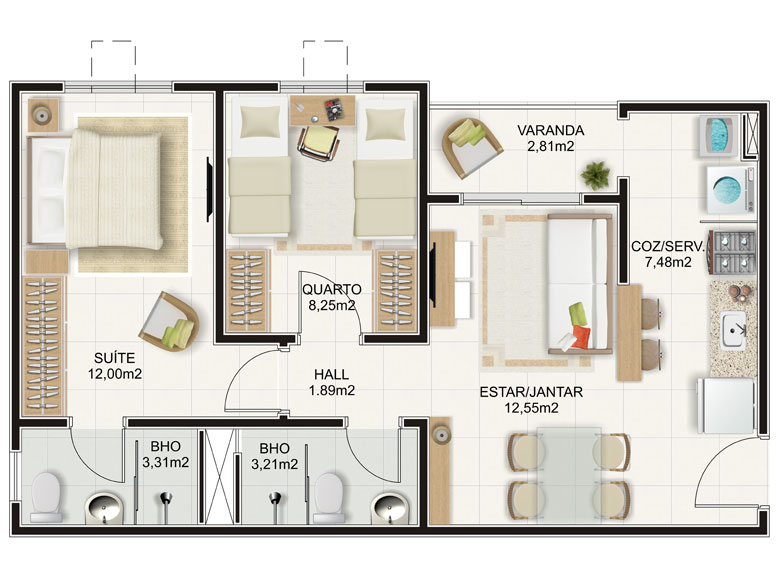
\includegraphics[width=13cm]{./02_Capitulos/02_Cap5/figures/planta-casa}
\caption{Planta baixa de residência de dois quartos, retirado de \cite{decorandocasas}}
\label{fig:5.1.0/planta-casa}
\end{figure}

Nota-se pela \ref{table:planta-casa}, com menos de R\$ 2000,00 pode-se instalar um sistema robusto para automatizar uma casa. O projeto já conta que a residência possui uma rede WiFi e se a casa tiver um PC, pode-se abater do custo do servidor.


\begin{table}[h!]
\centering
\caption{Orçamento de um sistema simples para automação da residência da \ref{fig:5.1.0/planta-casa}}
\begin{tabular}{|l|l|l|l|l|}
\hline
Item                & Descrição                    & Qtde & Unidade (R\$) & Total (R\$) \\ \hline
esp32               & Módulo de aquisição          & 4    & \$30.00       & \$120.00    \\ \hline
DHT11               & Sensor de temperatura        & 4    & \$10.00       & \$40.00     \\ \hline
P8                  & Módulo sensor de tensão      & 6    & \$20.00       & \$120.00    \\ \hline
Acs712 - 5a         & Módulo sensor de corrente    & 6    & \$15.00       & \$90.00     \\ \hline
Ssr-25              & Relé Estado Sólido           & 4    & \$30.00       & \$120.00    \\ \hline
Desktop             & Servidor Local               & 1    & \$600.00      & \$600.00    \\ \hline
Sensores Magnéticos & Sensores de abertura         & 6    & \$40.00       & \$240.00    \\ \hline
Infraestrura        & Caixas de proteção, fios etc & 1    & \$500.00      & \$500.00    \\ \hline
\multicolumn{4}{|l|}{TOTAL:}                                              & \$1,830.00  \\ \hline
\end{tabular}
\label{table:planta-casa}
\end{table}


\section{Aplicação: Controle de Iluminação de Postos de combustível}
\label{section:posto}


Essa é uma aplicação que pode ser usado no comércio assim como na indústria. Trata-se de uma central que controla via rede local as iluminações de postos de combustível. Estes possuem uma fonte de luz bastante potente na testeira(Parte de cima do posto) e no Totem (presente na entrada do posto, onde são mostrados os preços dos combustíveis). A infraestrutura do projeto não é complexa, Necessitará de um módulo ESP32 para processamento e envio dos acionamentos, relés de estado sólido, disjuntores de curva C, uma bateria que converte CA em CC, geralmente baterias similares as de celulares satisfazem, isso para o interfaciamento entre a rede elétrica e o sistema digital de controle. Por fim tudo isso ficará presente em uma caixa com vedação perto da caixa de energia do posto.

Para montar a rede Wifi local, será utilizado um roteador dedicado, configurando uma rede local, não é necessário a conexão a internet neste ponto do projeto. O ESP32 irá se conectar a rede por wps \cite{linksys}, O broker irá ser instalado em um desktop na parte administrativa do posto. O diferencial da aplicação está na aplicação. O frentista responsável poderá acessar a rede e um servidor HTTP irá fornecer uma página web no qual ele pode enviar comandos de acionamento das luzes e até agendar o acionamento destas para um horário específico.


\begin{table}[h]
\caption{Infraestrura para sistema de controle de iluminação de  postos de Combustíveis}
\begin{tabular}{|l|l|l|l|l|}
\hline
Item           & Descrição                   & Qtde & Unidade (R\$) & Total (R\$) \\ \hline
esp32          & Módulo de aquisição         & 1    & \$30.00       & \$30.00     \\ \hline
Disjuntor      & Curva C                     & 4    & \$40.00       & \$160.00    \\ \hline
P8             & Módulo sensor de tensão     & 6    & \$20.00       & \$120.00    \\ \hline
Acs712 - 5a    & Módulo sensor de corrente   & 6    & \$15.00       & \$90.00     \\ \hline
Ssr-25         & Relé Estado Sólido          & 4    & \$30.00       & \$120.00    \\ \hline
Desktop        & Servidor Local              & 1    & \$600.00      & \$600.00    \\ \hline
TP-Link AC1350 & Roteador Wireless           & 1    & \$280.00      & \$280.00    \\ \hline
Infraestrura   & Caixa de proteção, fios etc & 1    & \$700.00      & \$700.00    \\ \hline
\multicolumn{4}{|l|}{TOTAL}                                         & \$2,100.00  \\ \hline
\end{tabular}
\label{table:posto}
\end{table}		

Na \ref{table:posto}, como temos um sistema trifásico é necessário mais acionadores, como  as ferramentas utilizadas para o projeto da aplicação são de escopo aberto e gratuitas, não possuímos despesas neste aspecto. Deve-se planejar um local para que a caixa de controle consiga captar um sinal estável do roteador, e é recomendável configura-lo para enviar dados em um canal menos congestionado. O sensores de tensão e corrente foram adicionados caso seja adicionado ao projeto um monitoramento de consumo de energia.
\chapter{Estimativas de Custos}
\label{chapter:estimativa}

Para validar o baixo custo do sistema, este capítulo tem o foco em simular o orçamento de dois projetos. Um feito para a indústria e outro em redes domésticas para automações residenciais. Serão propostos cenários de aplicações reais, capazes de confirmar a premissa do projeto.
Como vimos no capítulo de projetos, o sistema pode ser instalado em plataformas mais sofisticadas, contendo sistemas operacionais e hardware dedicado. Mas nestes cenários utilizaremos o hardware mínimo que é compatível com o sistema e atua satisfatoriamente na aplicação.


\section{Aplicação: Automação Residencial}
\label{section:residencial}

O caso em estudo é a automação parcial de uma residência. Como pode ser visto em  \ref{fig:5.1.0/planta-casa}, a casa possui dois quartos, sala de estar, dois banheiros, cozinha, área de serviço e varanda. O objetivo é monitorar a temperatura local, o consumo de energia, detectar aberturas de portas e janelas de entrada da residência para fins de segurança e acionamento de luzes.

Para isso é necessário acionadores para a sala e cozinha, mais os quartos, totalizando cerca de 4 pontos de luz para acionar, o mesmo vale para os sensores de temperatura, no qual farão a média de temperatura da casa. Para controle de consumo de energia, nos limitaremos as tomadas de eletrodomésticos e eletrônicos, que representam a maior parte do consumo, para um ponto na sala, nos quartos, na tomada da geladeira, micro-ondas e lavadora, cerca de 6 tomadas a colocar sensores de tensão e corrente AC para cálculo da potência. Serão colocados sensores magnéticos para detectar abertura de portas e janelas, na porta de entrada, na porta da varanda, nas janelas do quarto e na área de serviço.

\begin{figure}[h!]
\centering
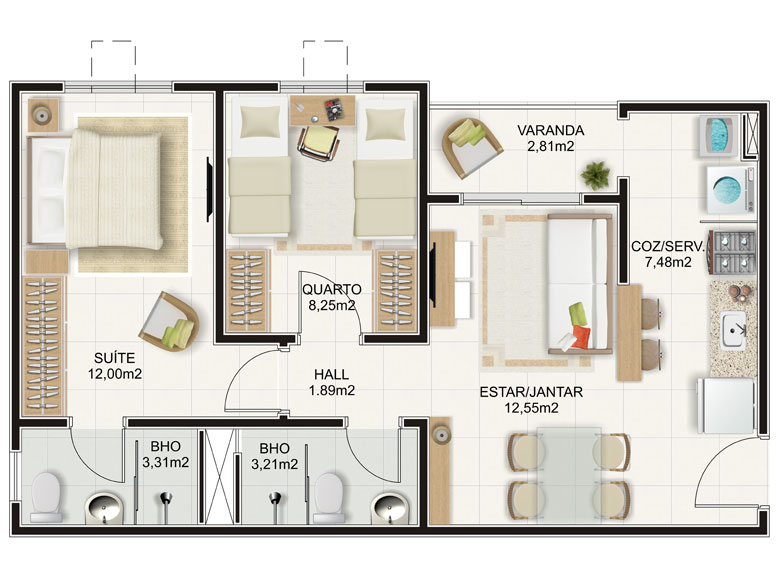
\includegraphics[width=13cm]{./02_Capitulos/02_Cap5/figures/planta-casa}
\caption{Planta baixa de residência de dois quartos, retirado de \cite{decorandocasas}}
\label{fig:5.1.0/planta-casa}
\end{figure}

Com menos de R\$ 2000,00 pode-se instalar um sistema robusto para automatizar uma casa. O projeto já conta que a residência possui uma rede WiFi e se a casa tiver um PC, pode-se abater do custo do servidor.


\begin{table}[h!]
\centering
\caption{Orçamento de um sistema simples para automação da residência da \ref{fig:5.1.0/planta-casa}}
\begin{tabular}{|l|l|l|l|l|}
\hline
Item                & Descrição                    & Qtde & Unidade (R\$) & Total (R\$) \\ \hline
esp32               & Módulo de aquisição          & 4    & \$30.00       & \$120.00    \\ \hline
DHT11               & Sensor de temperatura        & 4    & \$10.00       & \$40.00     \\ \hline
P8                  & Módulo sensor de tensão      & 6    & \$20.00       & \$120.00    \\ \hline
Acs712 - 5a         & Módulo sensor de corrente    & 6    & \$15.00       & \$90.00     \\ \hline
Ssr-25              & Relé Estado Sólido           & 4    & \$30.00       & \$120.00    \\ \hline
Desktop             & Servidor Local               & 1    & \$600.00      & \$600.00    \\ \hline
Sensores Magnéticos & Sensores de abertura         & 6    & \$40.00       & \$240.00    \\ \hline
Infraestrura        & Caixas de proteção, fios etc & 1    & \$500.00      & \$500.00    \\ \hline
\multicolumn{4}{|l|}{TOTAL:}                                              & \$1,830.00  \\ \hline
\end{tabular}
\label{table:planta-casa}
\end{table}




% inserir demais capítulos aqui
% -----------------------------
% -----------------------------
% -----------------------------
% -----------------------------





\pagebreak
\addcontentsline{toc}{chapter}{\hspace{1.7cm}\bfseries CONCLUSÃO}
\noindent\textbf{CONCLUSÃO}
$\!$\\


% Falar sobre o projeto em si
Nesta dissertação, foram apresentados todos os aspectos de hardware, software e econômicos em seus capítulos. Cada um explicando o planejamento a a forma de implementação da ideia, de modo a deixar claro ao leitor como construir e utilizar o sistema como um todo.

O sistema segue sua proposta de escopo aberto, escalável e de baixo custo. Foram apresentadas plataformas de hardware aberto, oferecendo a possibilidade de uma organização ou empresa distribuírem suas próprias versões e baratear ainda mais os custos em larga escala. Os softwares são de escopo aberto e licenças altamente permissíveis, o que significa que possuem versões gratuitas e escaláveis, de modo a também oferecerem a possibilidade de criar versões personalizadas.

A escolha de começar com aplicações feitas com base no TCP/IP, tornou o software flexível para a implementação de novos tipo de protocolos desta camada. Unido a grande quantidade de bibliotecas feitas em diversas linguagens de programação, o sistema pode ser escalado facilmente para aplicações específicas. O modelo Publish/Subscribe é um modelo que reúne características ideais para protocolos full-duplex, em transferências em tempo real, oferecendo a funcionalidade de cada dispositivo escolher quais dados desejam receber através do sistema de tópicos, oferecendo economia energética e de dados.

% Falar sobre intregação com clouds
Vale ressaltar sobre plataformas em nuvem que fornecem serviços IaaS, que podem ser inseridos nas camadas de IoT. Serviços como Brokers, Bancos de Dado, Autenticação, segurança, Inteligência Artificial, Análise e Visualização de dados, estão cada vez mais frequentes no universo do IoT. Isso facilita a implementação do sistema e podem oferecer soluções mais confiáveis e estáveis, porém isso aumenta o custo do sistema, pois esses serviços são pagos.

Por fim, este trabalho fornece uma porta para a Indústria 4.0, sobre Internet das Coisa e uma forma flexível de implementação de sistemas neste escopo. Para futuras funcionalidade, pode-se incluir ferramentas de segurança, integração com a cloud, outras implementações para bancos de dados e implementações da API em outras linguagens de programação.

\pagebreak





\pagebreak
\addcontentsline{toc}{chapter}{\hspace{1.7cm}\bfseries REFERÊNCIAS}
\def\bibname{REFERÊNCIAS}


%\nocite{*}
% abaixo segue a chamada para o arquivo [.BIB]. Utilizei o programa JABREF para montar o arquivo com minhas referências.
\bibliography{bib/dissertacao_folim}

\definecolor{light-gray}{gray}{0.97}


\chapter{Apêndice}
\label{chapter:apendice}

\section{Guias de instalação}
\label{section:guia}

\textbf{Atenção:} Para obter a versão mais atualizada e outras versões, acesse \url{https://github.com/fol21}. Este guia tem como objetivo reproduzir os testes feitos no sistema, realizados em distribuições de Windows 10 e Linux.

\subsection{Configurando Broker}
\label{subsection:guia_broker}

\begin{enumerate}

\item Acesse \url{https://mosquitto.org/download/} e siga as instruções para baixar e instalar o Mosquitto;
\item No terminal execute o comando \textit{mosquitto -d}
\item Use o IP e a porta configurada nos exemplos de Publisher e Subscriber;
\item Em C++ as configurações são encontradas no próprio código;
\item Em Javascript acesse o arquivo \textit{config.json} no diretório \textit{example/*/resources} e mude as configurações de IP e Porta;
\end{enumerate}

\subsection{Publishers em C++}
\label{subsection:guia_publishers_cpp}

\begin{enumerate}

\item Siga as instruções de instalação em \url{http://docs.platformio.org/en/latest/installation.html};
\item Acesse \url{https://docs.espressif.com/projects/esp-idf/en/latest/get-started/establish-serial-connection.html} e instale os drivers adequados para o ESP32;
\item Acesse \url{https://github.com/fol21/things-4-labs-acquirer-platform} e baixe o projeto;
\item No diretório do projeto digite os comandos \textit{pio run -t upload -e esp32};
\end{enumerate}

\subsection{Publishers em Javascript}
\label{subsection:guia_publishers_javascript}

\begin{enumerate}
\item Acesse \url{https://nodejs.org/en/} e baixe sua versão do Node.js na versão 8 ou maior;
\item Acesse \url{https://github.com/fol21/things-4-labs-acquirer-raspberrypi} e baixe o projeto;
\item Entre no diretório examples/gpio, presente no projeto;
\item Coloque as informações de IP e Porta no arquivo \textit{resources/config.json};
\item Execute o comando como administrador \textit{npm install};
\item Execute o comando como administrador \textit{node index.js};

\end{enumerate}


\subsection{Subscribers em Javascript}
\label{subsection:guia_subscribers_javascript}

\begin{enumerate}
\item Acesse \url{https://nodejs.org/en/} e baixe sua versão do Node.js na versão 8 ou maior;
\item Acesse \url{https://docs.mongodb.com/manual/installation/} e siga as instruções para instalar e iniciar o mongodb conforme seu Sistema Operacional;
\item Crie uma conta gratuita em \url{https://plot.ly/};
\item Acesse \url{https://github.com/fol21/things-4-labs-console-subscriber} e baixe o projeto;
\item Entre no diretório examples/simple-subscriber, presente no projeto;
\item Coloque as informações de IP e Porta no arquivo \textit{resources/config.json};
\item Coloque seu Id e chave da sua conta do Plotly em \textit{index.js};
\item Execute o comando como administrador \textit{npm install};
\item Execute o comando como administrador \textit{node index.js};

\end{enumerate}


\section{Códigos Fonte}
\label{section:codigos_fonte}

\textbf{Atenção:} Para obter a versão mais atualizada e outras versões, acesse \url{https://github.com/fol21}.

\subsection{Publishers em C++}
\label{subsection:publishers_cpp}


\lstinputlisting[language=C++,backgroundcolor= \color{light-gray}, caption=Data Stream Header, breaklines=true,basicstyle=\footnotesize\ttfamily]{./03_Conclusao/src/publisher-c++/data_stream.h}

\lstinputlisting[language=C++,backgroundcolor= \color{light-gray}, caption=Data Stream Source, breaklines=true,basicstyle=\footnotesize\ttfamily]{./03_Conclusao/src/publisher-c++/data_stream.cpp}

\lstinputlisting[language=C++,backgroundcolor= \color{light-gray}, caption=MQTT Publisher Header em C++, breaklines=true,basicstyle=\footnotesize\ttfamily]{./03_Conclusao/src/publisher-c++/MqttPublisher.h}

\lstinputlisting[language=C++,backgroundcolor= \color{light-gray}, caption=MQTT Publisher Source em C++, breaklines=true,basicstyle=\footnotesize\ttfamily]{./03_Conclusao/src/publisher-c++/MqttPublisher.cpp}



\subsection{Publishers em Javascript}
\label{subsection:publishers_javascript}


\lstinputlisting[language=C++,backgroundcolor= \color{light-gray}, caption=Data Stream em javascript, breaklines=true,basicstyle=\footnotesize\ttfamily]{./03_Conclusao/src/publisher-js/DataStream.js}

\lstinputlisting[language=C++,backgroundcolor= \color{light-gray}, caption=Continous Stream, breaklines=true,basicstyle=\footnotesize\ttfamily]{./03_Conclusao/src/publisher-js/ContinousStream.js}

\lstinputlisting[language=C++,backgroundcolor= \color{light-gray}, caption=Periodic Stream em Javascript, breaklines=true,basicstyle=\footnotesize\ttfamily]{./03_Conclusao/src/publisher-js/PeriodicStream.js}

\lstinputlisting[language=C++,backgroundcolor= \color{light-gray}, caption=MQTT Publisher Source em Javascript, breaklines=true,basicstyle=\footnotesize\ttfamily]{./03_Conclusao/src/publisher-js/MqttPublisher.js}

\lstinputlisting[language=C++,backgroundcolor= \color{light-gray}, caption=Index das implementações, breaklines=true,basicstyle=\footnotesize\ttfamily]{./03_Conclusao/src/publisher-js/index.js}


\subsection{Subscribers em Javascript}
\label{subsection:subscribers_javascript}

\lstinputlisting[language=C++,backgroundcolor= \color{light-gray}, caption=MQTT Subscriber Source em Javascript, breaklines=true,basicstyle=\footnotesize\ttfamily]{./03_Conclusao/src/subscriber-js/MqttSubscriber.js}

\lstinputlisting[language=C++,backgroundcolor= \color{light-gray}, caption=Index das implementações, breaklines=true,basicstyle=\footnotesize\ttfamily]{./03_Conclusao/src/subscriber-js/index.js}

\lstinputlisting[language=C++,backgroundcolor= \color{light-gray}, caption=Data Client para MongoDB, breaklines=true,basicstyle=\footnotesize\ttfamily]{./03_Conclusao/src/subscriber-js/MongoDataClient.js}

\subsection{Códigos fonte das aplicações em consoles}
\label{subsection:teste_fonte}


\lstinputlisting[language=C++,backgroundcolor= \color{light-gray}, caption= Teste do publisher, breaklines=true,basicstyle=\footnotesize\ttfamily]{./03_Conclusao/src/publisher-js/example.js}

\lstinputlisting[language=C++,backgroundcolor= \color{light-gray}, caption=Teste do subscriber, breaklines=true,basicstyle=\footnotesize\ttfamily]{./03_Conclusao/src/subscriber-js/example.js}

\subsection{Códigos fonte das aplicações em plataformas embarcadas}
\label{subsection:teste-plataformas}


\lstinputlisting[language=C++,backgroundcolor= \color{light-gray}, caption= Teste do publisher no ESP32, breaklines=true,basicstyle=\footnotesize\ttfamily]{./03_Conclusao/src/publisher-c++/main.cpp}




% \printindex    %Removi o índice remissivo para a versão oficial do trabalho.


\end{document}